

%%%%%%%%%%%%%%%%%%%%%%%%%%%%%%%%%%%%%%%%%%%%%%%%%%%%%%%%%%%%%%%%%%%%%%
%%%%%%%%%%%%%%%% Deep Learning with label noise
%%%%%%%%%%%%%%%%%%%%%%%%%%%%%%%%%%%%%%%%%%%%%%%%%%%%%%%%%%%%%%%%%%%%%%

\section{Deep Learning with Label Noises}

%%%%%%%% To clarify inputs independence and spatial independence of noises

\subsection{Label noises}
Label noises can be categories into three statistical models, noisy complete at random (NCAR), noisy at random (NAR) and noisy not at random (NNAR), based on whether label noises depends on classes and distribution of inputs. (Figure \ref{fig:noises})
For noisy completely at random models, the occurrence of an error $E$ is independent of neither the true class $Y$ nor the input $X$.
Noisy at random models are similar to NCAR models except that the label noise is asymmetric, meaning it depends on classes.
The NAR model can be interpreted in terms of a transition (or confusion) matrix:
\[
\gamma =
\begin{bmatrix}
    P(Y^{\ast}=1\vert Y=1)   & \dots  & P(Y^{\ast}=n_y\vert Y=1) \\
    \vdots                   & \ddots & \vdots \\
    P(Y^{\ast}=1\vert Y=n_y) & \dots  & P(Y^{\ast}=n_y\vert Y=n_y)
\end{bmatrix}
\]
where $Y^{\ast}$ is a random variable for observed label and $Y$ is another variable for true label.
NNAR:

\begin{figure}[t]
\begin{center}
% \fbox{\rule{0pt}{2in} \rule{0.9\linewidth}{0pt}}
   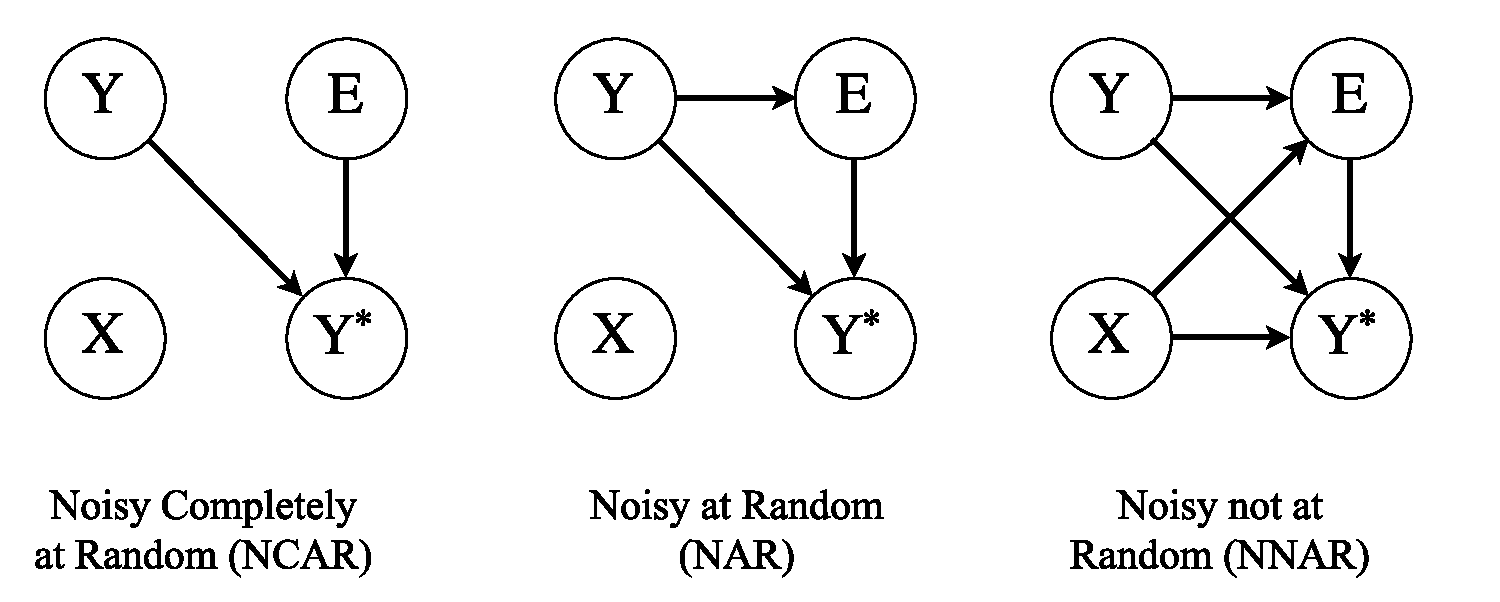
\includegraphics[width=1.05\linewidth]{img/label_noises}
\end{center}
   \caption{
   Graphical models for three types of label noises. \cite{frenay2014classification}
   The graphical models describe if the probability of the errorness and observed value of a label conditions on the true class and inputs.
   }
\label{fig:noises}
\end{figure}
